\documentclass[]{article}
\usepackage{lmodern}
\usepackage{amssymb,amsmath}
\usepackage{ifxetex,ifluatex}
\usepackage{fixltx2e} % provides \textsubscript
\ifnum 0\ifxetex 1\fi\ifluatex 1\fi=0 % if pdftex
  \usepackage[T1]{fontenc}
  \usepackage[utf8]{inputenc}
\else % if luatex or xelatex
  \ifxetex
    \usepackage{mathspec}
  \else
    \usepackage{fontspec}
  \fi
  \defaultfontfeatures{Ligatures=TeX,Scale=MatchLowercase}
\fi
% use upquote if available, for straight quotes in verbatim environments
\IfFileExists{upquote.sty}{\usepackage{upquote}}{}
% use microtype if available
\IfFileExists{microtype.sty}{%
\usepackage{microtype}
\UseMicrotypeSet[protrusion]{basicmath} % disable protrusion for tt fonts
}{}
\usepackage[margin=1in]{geometry}
\usepackage{hyperref}
\hypersetup{unicode=true,
            pdftitle={Laborator 3},
            pdfborder={0 0 0},
            breaklinks=true}
\urlstyle{same}  % don't use monospace font for urls
\usepackage{color}
\usepackage{fancyvrb}
\newcommand{\VerbBar}{|}
\newcommand{\VERB}{\Verb[commandchars=\\\{\}]}
\DefineVerbatimEnvironment{Highlighting}{Verbatim}{commandchars=\\\{\}}
% Add ',fontsize=\small' for more characters per line
\usepackage{framed}
\definecolor{shadecolor}{RGB}{248,248,248}
\newenvironment{Shaded}{\begin{snugshade}}{\end{snugshade}}
\newcommand{\KeywordTok}[1]{\textcolor[rgb]{0.13,0.29,0.53}{\textbf{#1}}}
\newcommand{\DataTypeTok}[1]{\textcolor[rgb]{0.13,0.29,0.53}{#1}}
\newcommand{\DecValTok}[1]{\textcolor[rgb]{0.00,0.00,0.81}{#1}}
\newcommand{\BaseNTok}[1]{\textcolor[rgb]{0.00,0.00,0.81}{#1}}
\newcommand{\FloatTok}[1]{\textcolor[rgb]{0.00,0.00,0.81}{#1}}
\newcommand{\ConstantTok}[1]{\textcolor[rgb]{0.00,0.00,0.00}{#1}}
\newcommand{\CharTok}[1]{\textcolor[rgb]{0.31,0.60,0.02}{#1}}
\newcommand{\SpecialCharTok}[1]{\textcolor[rgb]{0.00,0.00,0.00}{#1}}
\newcommand{\StringTok}[1]{\textcolor[rgb]{0.31,0.60,0.02}{#1}}
\newcommand{\VerbatimStringTok}[1]{\textcolor[rgb]{0.31,0.60,0.02}{#1}}
\newcommand{\SpecialStringTok}[1]{\textcolor[rgb]{0.31,0.60,0.02}{#1}}
\newcommand{\ImportTok}[1]{#1}
\newcommand{\CommentTok}[1]{\textcolor[rgb]{0.56,0.35,0.01}{\textit{#1}}}
\newcommand{\DocumentationTok}[1]{\textcolor[rgb]{0.56,0.35,0.01}{\textbf{\textit{#1}}}}
\newcommand{\AnnotationTok}[1]{\textcolor[rgb]{0.56,0.35,0.01}{\textbf{\textit{#1}}}}
\newcommand{\CommentVarTok}[1]{\textcolor[rgb]{0.56,0.35,0.01}{\textbf{\textit{#1}}}}
\newcommand{\OtherTok}[1]{\textcolor[rgb]{0.56,0.35,0.01}{#1}}
\newcommand{\FunctionTok}[1]{\textcolor[rgb]{0.00,0.00,0.00}{#1}}
\newcommand{\VariableTok}[1]{\textcolor[rgb]{0.00,0.00,0.00}{#1}}
\newcommand{\ControlFlowTok}[1]{\textcolor[rgb]{0.13,0.29,0.53}{\textbf{#1}}}
\newcommand{\OperatorTok}[1]{\textcolor[rgb]{0.81,0.36,0.00}{\textbf{#1}}}
\newcommand{\BuiltInTok}[1]{#1}
\newcommand{\ExtensionTok}[1]{#1}
\newcommand{\PreprocessorTok}[1]{\textcolor[rgb]{0.56,0.35,0.01}{\textit{#1}}}
\newcommand{\AttributeTok}[1]{\textcolor[rgb]{0.77,0.63,0.00}{#1}}
\newcommand{\RegionMarkerTok}[1]{#1}
\newcommand{\InformationTok}[1]{\textcolor[rgb]{0.56,0.35,0.01}{\textbf{\textit{#1}}}}
\newcommand{\WarningTok}[1]{\textcolor[rgb]{0.56,0.35,0.01}{\textbf{\textit{#1}}}}
\newcommand{\AlertTok}[1]{\textcolor[rgb]{0.94,0.16,0.16}{#1}}
\newcommand{\ErrorTok}[1]{\textcolor[rgb]{0.64,0.00,0.00}{\textbf{#1}}}
\newcommand{\NormalTok}[1]{#1}
\usepackage{longtable,booktabs}
\usepackage{graphicx,grffile}
\makeatletter
\def\maxwidth{\ifdim\Gin@nat@width>\linewidth\linewidth\else\Gin@nat@width\fi}
\def\maxheight{\ifdim\Gin@nat@height>\textheight\textheight\else\Gin@nat@height\fi}
\makeatother
% Scale images if necessary, so that they will not overflow the page
% margins by default, and it is still possible to overwrite the defaults
% using explicit options in \includegraphics[width, height, ...]{}
\setkeys{Gin}{width=\maxwidth,height=\maxheight,keepaspectratio}
\IfFileExists{parskip.sty}{%
\usepackage{parskip}
}{% else
\setlength{\parindent}{0pt}
\setlength{\parskip}{6pt plus 2pt minus 1pt}
}
\setlength{\emergencystretch}{3em}  % prevent overfull lines
\providecommand{\tightlist}{%
  \setlength{\itemsep}{0pt}\setlength{\parskip}{0pt}}
\setcounter{secnumdepth}{5}
% Redefines (sub)paragraphs to behave more like sections
\ifx\paragraph\undefined\else
\let\oldparagraph\paragraph
\renewcommand{\paragraph}[1]{\oldparagraph{#1}\mbox{}}
\fi
\ifx\subparagraph\undefined\else
\let\oldsubparagraph\subparagraph
\renewcommand{\subparagraph}[1]{\oldsubparagraph{#1}\mbox{}}
\fi

%%% Use protect on footnotes to avoid problems with footnotes in titles
\let\rmarkdownfootnote\footnote%
\def\footnote{\protect\rmarkdownfootnote}

%%% Change title format to be more compact
\usepackage{titling}

% Create subtitle command for use in maketitle
\newcommand{\subtitle}[1]{
  \posttitle{
    \begin{center}\large#1\end{center}
    }
}

\setlength{\droptitle}{-2em}

  \title{Laborator 3}
    \pretitle{\vspace{\droptitle}\centering\huge}
  \posttitle{\par}
  \subtitle{Elemente de probabilități în R}
  \author{}
    \preauthor{}\postauthor{}
    \date{}
    \predate{}\postdate{}
  
\usepackage{booktabs}
\usepackage{longtable}
\usepackage{framed,color}
\definecolor{shadecolor}{RGB}{248, 248, 248}
\definecolor{shadecolor1}{RGB}{216,225,235}
\definecolor{framecolor}{RGB}{16,111,124}%108,123,13

%\definecolor{shadecolor}{RGB}{226, 255, 241}
% \definecolor{shadecolor1}{RGB}{217,225,199}
% \definecolor{framecolor}{RGB}{60,179,113}

%%%%%%%%%%%%%%%%%%%%%%
\ifxetex
  \usepackage{letltxmacro}
  \setlength{\XeTeXLinkMargin}{1pt}
  \LetLtxMacro\SavedIncludeGraphics\includegraphics
  \def\includegraphics#1#{% #1 catches optional stuff (star/opt. arg.)
    \IncludeGraphicsAux{#1}%
  }%
  \newcommand*{\IncludeGraphicsAux}[2]{%
    \XeTeXLinkBox{%
      \SavedIncludeGraphics#1{#2}%
    }%
  }%
\fi

\newenvironment{frshaded*}{%
  \def\FrameCommand{\fboxrule=\FrameRule\fboxsep=\FrameSep \fcolorbox{framecolor}{shadecolor1}}%
  \MakeFramed {\advance\hsize-\width \FrameRestore}}%
{\endMakeFramed}

\newenvironment{rmdblock}[1]
  {\begin{frshaded*}
  \begin{itemize}
  \renewcommand{\labelitemi}{
    \raisebox{-.7\height}[0pt][0pt]{
      {\setkeys{Gin}{width=2em,keepaspectratio}\includegraphics{images/icons/#1}}
    }
  }
  \item
  }
  {
  \end{itemize}
  \end{frshaded*}
  }
  
%%%%%%%%%%%%%%%
% definitions.
% -------------------
\usepackage{marginnote}
% \renewcommand*{\marginnotevadjust}{40pt}
% \renewcommand{\marginnotevadjust}{0pt}
% \renewcommand{\marginfont}{\noindent\rule{0pt}{0.7\baselineskip}\tiny}

\newtheorem{proposition}{Proposition}[section]
\newtheorem{lemma}[proposition]{Lemma}
\newtheorem{corollary}[proposition]{Corollary}
\newtheorem{theorem}[proposition]{Theorem}

\newcounter{exo}[section]
\newcommand{\enonce}[2]{\refstepcounter{proposition}\hypertarget{exo:#1}{}\label{exo:#1}{\scriptsize\;\textbf{Ex.}~\ref{exo:#1}}}

\reversemarginpar
\setlength{\marginparwidth}{1.2cm}
% 
% \newcommand{\enonce}[2]{\refstepcounter{proposition}\hypertarget{exo:#1}{}\label{exo:#1}{\noindent\color{black}\normalsize\bf Exercice \ref{exo:#1}}\ \  #2\vspace{1mm}\hrule\vspace{1mm} \color{black}\normalsize}


%%%%%%%%%%%%%%%

% \newenvironment{rmdcaution}
%   {\begin{rmdblock}{caution}}
%   {\end{rmdblock}}

% \newenvironment{rmdinsight}
%   {\begin{rmdblock}{insight}}
%   {\end{rmdblock}}

\newenvironment{rmdexercise}
  {\begin{rmdblock}{exercise}}
  {\end{rmdblock}}

% \newenvironment{rmdexercise_tex}
%   {\begin{rmdblock}{exercise}}
%   {\end{rmdblock}}
  
% \newenvironment{rmdtip}
%   {\begin{rmdblock}{tip}}
%   {\end{rmdblock}}


%%%%%%%%%%%%%%%%%%%%%%%%%%%%%%%%%%%%%%%%%%%%%%%%%%%%%%%%%%%%%%%%%%%%%%%%%%%%%%%%%%%%%%%%%%%%%%%%%%%%%%%%%%%%%%%%%%%%%
%%%%%%%%%%% For insight block %%%%%%%%%%%%%%%%%%%%%%%%%%
\definecolor{shadecolor_insight}{RGB}{223,240,216}
\definecolor{framecolor_insight}{RGB}{136,193,137}

%\definecolor{shadecolor_insight}{RGB}{217,225,199}
%\definecolor{framecolor_insight}{RGB}{60,179,113}

\newenvironment{frshaded_insight*}{%
  \def\FrameCommand{\fboxrule=\FrameRule\fboxsep=\FrameSep \fcolorbox{framecolor_insight}{shadecolor_insight}}%
  \MakeFramed {\advance\hsize-\width \FrameRestore}}%
{\endMakeFramed}

\newenvironment{rmdblock_insight}[1]
  {\begin{frshaded_insight*}
  \begin{itemize}
  \renewcommand{\labelitemi}{
    \raisebox{-.7\height}[0pt][0pt]{
      {\setkeys{Gin}{width=2em,keepaspectratio}\includegraphics{images/icons/#1}}
    }
  }
  \item
  }
  {
  \end{itemize}
  \end{frshaded_insight*}
  }

\newenvironment{rmdinsight}
  {\begin{rmdblock_insight}{insight}}
  {\end{rmdblock_insight}}

%%%%%%%%%%% For caution block %%%%%%%%%%%%%%%%%%%%%%%%%%
\definecolor{shadecolor_caution}{RGB}{250,250,250}
\definecolor{framecolor_caution}{RGB}{242,129,67}%193,75,34

\newenvironment{frshaded_caution*}{%
  \def\FrameCommand{\fboxrule=\FrameRule\fboxsep=\FrameSep \fcolorbox{framecolor_caution}{shadecolor_caution}}%
  \MakeFramed {\advance\hsize-\width \FrameRestore}}%
{\endMakeFramed}

\newenvironment{rmdblock_caution}[1]
  {\begin{frshaded_caution*}
  \begin{itemize}
  \renewcommand{\labelitemi}{
    \raisebox{-.7\height}[0pt][0pt]{
      {\setkeys{Gin}{width=2em,keepaspectratio}\includegraphics{images/icons/#1}}
    }
  }
  \item
  }
  {
  \end{itemize}
  \end{frshaded_caution*}
  }
  
\newenvironment{rmdcaution}
  {\begin{rmdblock_caution}{caution}}
  {\end{rmdblock_caution}}

%%%%%%%%%%% For tip block %%%%%%%%%%%%%%%%%%%%%%%%%%
\definecolor{shadecolor_tip}{RGB}{250,250,250}
\definecolor{framecolor_tip}{RGB}{33,153,195}

\newenvironment{frshaded_tip*}{%
  \def\FrameCommand{\fboxrule=\FrameRule\fboxsep=\FrameSep \fcolorbox{framecolor_tip}{shadecolor_tip}}%
  \MakeFramed {\advance\hsize-\width \FrameRestore}}%
{\endMakeFramed}

\newenvironment{rmdblock_tip}[1]
  {\begin{frshaded_tip*}
  \begin{itemize}
  \renewcommand{\labelitemi}{
    \raisebox{-.7\height}[0pt][0pt]{
      {\setkeys{Gin}{width=2em,keepaspectratio}\includegraphics{images/icons/#1}}
    }
  }
  \item
  }
  {
  \end{itemize}
  \end{frshaded_tip*}
  }
  
\newenvironment{rmdtip}
  {\begin{rmdblock_tip}{tip}}
  {\end{rmdblock_tip}}

%%%%%%%%%%%%%%%%%%%%%%%%%%%%%%%%%%%%%%%%%%%%%%%%%%%%%%%%%%%%%%%%%%%%%%%%%%%%%%%%%%%%%%%%%%%%%%%%%%%%%%%%%%%%%%%%%%%%%
\usepackage{subfigure}
\usepackage{booktabs}
\usepackage{slashbox}
\usepackage{color}
%%%%%%%%%%%%%%%%%%%%%%%%%%%%%%%%%%%%%%%%%
\definecolor{linkcol}{rgb}{0,0,0.4}
\definecolor{citecol}{rgb}{0.5,0,0}

% Change this to change the informations included in the pdf file
% \usepackage[pagebackref]{hyperref}
% \usepackage[verbose]{backref}
\usepackage[hyperpageref]{backref}
% \backrefsetup{verbose=false}
% \PassOptionsToPackage{pagebackref}{hyperref}
% See hyperref documentation for information on those parameters

\hypersetup
{
bookmarksopen=true,
pdftitle="Curs Probabilitati si Statistica",
pdfauthor="Alexandru Amarioarei",
pdfsubject="Curs Probabilitati si Statistica", %subject of the document
pdfmenubar=true, %menubar shown
pdfhighlight=/O, %effect of clicking on a link
colorlinks=true, %couleurs sur les liens hypertextes
pdfpagemode=None, %aucun mode de page
pdfpagelayout=SinglePage, %ouverture en simple page
pdffitwindow=true, %pages ouvertes entierement dans toute la fenetre
linkcolor=linkcol, %couleur des liens hypertextes internes
citecolor=citecol, %couleur des liens pour les citations
urlcolor=linkcol %couleur des liens pour les url
}


% set the back references
\renewcommand*{\backref}[1]{}
\renewcommand*{\backreftwosep}{ și~} % inserted between entries 
                              % in a list of two entries, 
                              % default is " and~".
\renewcommand*{\backreflastsep}{ și~} % inserted between the last 
                               % two entries of a list with more
                               % than two entries, default is ", and~".
\renewcommand*{\backrefalt}[4]{%
    \ifcase #1 (Necitat.)%
    \or        (Citat la pagina~#2.)%
    \else      (Citat la paginile~#2.)%
    \fi}

%%%%%%%%%%%%%%%%%%%%%%%%%%%%%%%%%%%%%%%%%%%%%%%%%%%%%%%%%%%%%%%%%%%%%%%%%%%%%%%%%%%%%%%%%%%%%%%%%%%%%%%%%%%%%%%%%%%%%
%CITEVA DEFINITII
\def\om{\omega}
\def\Om{\Omega}
\def\et{\eta}
\def\td{\tilde{\delta}}
\def\m{{\mu}}
\def\n{{\nu}}
\def\k{{\kappa}}
\def\l{{\lambda}}
\def\L{{\Lambda}}
\def\g{{\gamma}}
\def\a{{\alpha}}
\def\e{{\varepsilon}}
\def\b{{\beta}}
\def\G{{\Gamma}}
\def\d{{\delta}}
\def\D{{\Delta}}
\def\t{{\theta}}
\def\s{{\sigma}}
\def\S{{\Sigma}}
\def\z{{\zeta}}
\def\qed{\hfill\Box}
\def\ds{\displaystyle}
\def\mc{\mathcal}
%%%%%%%%%%%%%%%%%%%%%%%%%%%%%%%%%%%%%%%%%%%%%%%%%%%%%%%%%%%%%%%%%%%%%%%%%%%%%%%%%%%%%%%%%%%%%%%%%%%%%%%%%%%%%%%%%%%%%%
\def\1{{\mathbf 1}}
\def\CC{{\mathbb C}}
\def\VV{{\mathbb V}}
\def\RR{{\mathbb R}}
\def\QQ{{\mathbb Q}}
\def\ZZ{{\mathbb Z}}
\def\PP{{\mathbb P}}
\def\EE{{\mathbb E}}
\def\NN{{\mathbb N}}
\def\FF{{\mathbb F}}
%\def\SS{{\mathbb S}}
\def\MA{{\mathcal A}}
\def\MO{{\mathcal O}}
\def\MF{{\mathcal F}}
\def\ME{{\mathcal E}}
\def\MR{{\mathcal R}}
\def\MB{{\mathcal B}}
\def\MM{{\mathcal M}}
\def\MN{{\mathcal N}}
\def\MU{{\mathcal U}}
\def\MP{{\mathcal P}}
\def\MS{{\mathcal S}}
\def\MBS{{\mathbf S}}
\def\MX{{\bm{ \mathscr X}}}

% independent sign
\newcommand\independent{\protect\mathpalette{\protect\independenT}{\perp}}
\def\independenT#1#2{\mathrel{\rlap{$#1#2$}\mkern2mu{#1#2}}}

\renewcommand\tablename{Tab.}
\renewcommand{\figurename}{Fig.}
\renewcommand\refname{Referințe}

%%%%%%%%%%%%%%%%%%%%%%%%%%%%%%%%%%%%%%%%%%%%%%%%%%%%%%%%%%%%%%%%%%%%%%%%%%%%%%%%%%%%%%%%%%%%%%%%%%%%%%%%%%%%%%%%%%%%%
%Header and Footer
\usepackage{fancyhdr}

\pagestyle{fancy}
\fancyhf{}
\rhead{Universitatea din Bucure\c sti\\ Facultatea de Matematic\u a \c si Informatic\u a}
% \lhead{\textit{Curs}: Tehnici alternative în predarea matematicii (2018)\\ \textit{Instructori}: A. Am\u arioarei, M. Patriche}
\lhead{\textit{Curs}: Probabilități și Statistică (2018-2019)\\ \textit{Instructor}: A. Am\u arioarei}
\rfoot{Pagina \thepage}
\lfoot{Grupele: 241, 242, 243, 244}
%%%%%%%%%%%%%%%%%%%%%%%%%%%%%%%%%%%%%%%
%%%%%%%%%%%%%%%%%%%%%%%%%%%%%%%%%%%%%%%
\usepackage{pifont}% http://ctan.org/pkg/pifont
\newcommand{\cmark}{\ding{51}}%
\newcommand{\xmark}{\ding{55}}%
\usepackage{booktabs}
\usepackage{longtable}
\usepackage{array}
\usepackage{multirow}
\usepackage[table]{xcolor}
\usepackage{wrapfig}
\usepackage{float}
\usepackage{colortbl}
\usepackage{pdflscape}
\usepackage{tabu}
\usepackage{threeparttable}
\usepackage{threeparttablex}
\usepackage[normalem]{ulem}
\usepackage{makecell}

\begin{document}
\maketitle

%%%%%%%%%%%%%%%%%%%%%%%%
\thispagestyle{fancy}

Obiectivul acestui laborator este de a prezenta succint câteva funcții
utile teoriei probabilităților din programul
\href{https://cran.r-project.org/}{R}, care este structura lor și cum le
putem aplica. De asemenea, tot în acest laborator vom prezenta și câteva
probleme ce se pot rezolva cu ajutorul algoritmilor aleatori.

\section{\texorpdfstring{Familia de funcții
\texttt{apply}}{Familia de funcții apply}}\label{familia-de-functii-apply}

Pe lângă buclele \texttt{for} și \texttt{while}, în R există și un set
de funcții care permit scrierea și rularea într-o manieră mai compactă a
codului dar și aplicarea de funcții unor grupuri de date.

\begin{itemize}
\item
  \texttt{lapply()}: Evaluează o funcție pentru fiecare element al unei
  liste
\item
  \texttt{sapply()}: La fel ca \texttt{lapply} numai că încearcă să
  simplifice rezultatul
\item
  \texttt{apply()}: Aplică o funcție după fiecare dimensiune a unui
  \texttt{array}
\item
  \texttt{tapply()}: Aplică o funcție pe submulțimi ale unui vector
\item
  \texttt{mapply()}: Varianta multivariată a funcției \texttt{lapply}
\item
  \texttt{split}: Împarte un vector în grupuri definite de o variabilă
  de tip factor.
\end{itemize}

\subsection{\texorpdfstring{\texttt{lapply()}}{lapply()}}\label{lapply}

Funcția \texttt{lapply()} efectuează următoarele operații:

\begin{enumerate}
\def\labelenumi{\arabic{enumi}.}
\tightlist
\item
  buclează după o listă, iterând după fiecare element din acea listă
\item
  aplică o \emph{funcție} fiecărui element al listei (o funcție pe care
  o specificăm)
\item
  întoarce ca rezultat tot o listă (prefixul \texttt{l} vine de la
  listă).
\end{enumerate}

Această funcție primește următoarele trei argument: (1) o listă
\texttt{X}; (2) o funcție \texttt{FUN}; (3) alte argumente via
\texttt{...}. Dacă \texttt{X} nu este o listă atunci aceasta va fi
transformată într-una folosind comanda \texttt{as.list()}.

Considerăm următorul exemplu în care vrem să aplicăm funcția
\texttt{mean()} tuturor elementelor unei liste

\begin{Shaded}
\begin{Highlighting}[]
\KeywordTok{set.seed}\NormalTok{(}\DecValTok{222}\NormalTok{)}
\NormalTok{x <-}\StringTok{ }\KeywordTok{list}\NormalTok{(}\DataTypeTok{a =} \DecValTok{1}\OperatorTok{:}\DecValTok{5}\NormalTok{, }\DataTypeTok{b =} \KeywordTok{rnorm}\NormalTok{(}\DecValTok{10}\NormalTok{), }\DataTypeTok{c =} \KeywordTok{rnorm}\NormalTok{(}\DecValTok{20}\NormalTok{, }\DecValTok{1}\NormalTok{), }\DataTypeTok{d =} \KeywordTok{rnorm}\NormalTok{(}\DecValTok{100}\NormalTok{, }\DecValTok{5}\NormalTok{))}
\KeywordTok{lapply}\NormalTok{(x, mean)}
\OperatorTok{$}\NormalTok{a}
\NormalTok{[}\DecValTok{1}\NormalTok{] }\DecValTok{3}

\OperatorTok{$}\NormalTok{b}
\NormalTok{[}\DecValTok{1}\NormalTok{] }\FloatTok{0.1996044}

\OperatorTok{$}\NormalTok{c}
\NormalTok{[}\DecValTok{1}\NormalTok{] }\FloatTok{0.7881026}

\OperatorTok{$}\NormalTok{d}
\NormalTok{[}\DecValTok{1}\NormalTok{] }\FloatTok{5.064188}
\end{Highlighting}
\end{Shaded}

Putem să folosim funcția \texttt{lapply()} pentru a evalua o funcție în
moduri repetate. Mai jos avem un exemplu în care folosim funcția
\texttt{runif()} (permite generarea observațiilor uniform repartizate)
de patru ori, de fiecare dată generăm un număr diferit de valori
aleatoare. Mai mult, argumentele \(min=0\) și \(max=3\) sunt atribuite,
prin intermediul argumentului \texttt{...}, funcției \texttt{runif}.

\begin{Shaded}
\begin{Highlighting}[]
\NormalTok{x <-}\StringTok{ }\DecValTok{1}\OperatorTok{:}\DecValTok{4}
\KeywordTok{lapply}\NormalTok{(x, runif, }\DataTypeTok{min =} \DecValTok{0}\NormalTok{, }\DataTypeTok{max =} \DecValTok{3}\NormalTok{)}
\NormalTok{[[}\DecValTok{1}\NormalTok{]]}
\NormalTok{[}\DecValTok{1}\NormalTok{] }\FloatTok{0.03443616}

\NormalTok{[[}\DecValTok{2}\NormalTok{]]}
\NormalTok{[}\DecValTok{1}\NormalTok{] }\FloatTok{1.267361} \FloatTok{1.365441}

\NormalTok{[[}\DecValTok{3}\NormalTok{]]}
\NormalTok{[}\DecValTok{1}\NormalTok{] }\FloatTok{1.8084700} \FloatTok{2.1902665} \FloatTok{0.4139585}

\NormalTok{[[}\DecValTok{4}\NormalTok{]]}
\NormalTok{[}\DecValTok{1}\NormalTok{] }\FloatTok{1.5924650} \FloatTok{0.7355067} \FloatTok{2.1483841} \FloatTok{1.6082945}
\end{Highlighting}
\end{Shaded}

\subsection{\texorpdfstring{\texttt{sapply()}}{sapply()}}\label{sapply}

Funcția \texttt{sapply()} are un comportament similar cu
\texttt{lapply()} prin faptul că funcția \texttt{sapply()} apelează
intern \texttt{lapply()} pentru valorile de input, după care evaluează:

\begin{itemize}
\item
  dacă rezultatul este o listă în care fiecare element este de lungime
  1, atunci întoarce un vector
\item
  dacă rezultatul este o listă în care fiecare element este un vector de
  aceeași lungime (\textgreater{}1), se întoarce o matrice
\item
  în caz contrar se întoarce o listă.
\end{itemize}

Considerăm exemplul de mai sus

\begin{Shaded}
\begin{Highlighting}[]
\KeywordTok{set.seed}\NormalTok{(}\DecValTok{222}\NormalTok{)}
\NormalTok{x <-}\StringTok{ }\KeywordTok{list}\NormalTok{(}\DataTypeTok{a =} \DecValTok{1}\OperatorTok{:}\DecValTok{4}\NormalTok{, }\DataTypeTok{b =} \KeywordTok{rnorm}\NormalTok{(}\DecValTok{10}\NormalTok{), }\DataTypeTok{c =} \KeywordTok{rnorm}\NormalTok{(}\DecValTok{20}\NormalTok{, }\DecValTok{1}\NormalTok{), }\DataTypeTok{d =} \KeywordTok{rnorm}\NormalTok{(}\DecValTok{100}\NormalTok{, }\DecValTok{5}\NormalTok{))}
\KeywordTok{sapply}\NormalTok{(x, mean)}
\NormalTok{        a         b         c         d }
\FloatTok{2.5000000} \FloatTok{0.1996044} \FloatTok{0.7881026} \FloatTok{5.0641876} 
\end{Highlighting}
\end{Shaded}

\subsection{\texorpdfstring{\texttt{split()}}{split()}}\label{split}

Funcția \texttt{split()} primește ca argument un vector sau o listă (sau
un data.frame) și împarte datele în grupuri determinate de o variabilă
de tip factor (sau o listă de factor).

Argumentele aceste funcții sunt

\begin{Shaded}
\begin{Highlighting}[]
\KeywordTok{str}\NormalTok{(split)}
\ControlFlowTok{function}\NormalTok{ (x, f, }\DataTypeTok{drop =} \OtherTok{FALSE}\NormalTok{, ...)  }
\end{Highlighting}
\end{Shaded}

unde

\begin{itemize}
\tightlist
\item
  \texttt{x} este un vector, o listă sau un data.frame
\item
  \texttt{f} este un factor sau o listă de factori
\end{itemize}

Considerăm următorul exemplu în care generăm un vector de date și îl
împărțim după o variabilă de tip factor creată cu ajutorul funcției
\texttt{gl()} (\emph{generate levels}).

\begin{Shaded}
\begin{Highlighting}[]
\NormalTok{x <-}\StringTok{ }\KeywordTok{c}\NormalTok{(}\KeywordTok{rnorm}\NormalTok{(}\DecValTok{10}\NormalTok{), }\KeywordTok{runif}\NormalTok{(}\DecValTok{10}\NormalTok{), }\KeywordTok{rnorm}\NormalTok{(}\DecValTok{10}\NormalTok{, }\DecValTok{1}\NormalTok{))}
\NormalTok{f <-}\StringTok{ }\KeywordTok{gl}\NormalTok{(}\DecValTok{3}\NormalTok{, }\DecValTok{10}\NormalTok{)}
\KeywordTok{split}\NormalTok{(x, f)}
\OperatorTok{$}\StringTok{`}\DataTypeTok{1}\StringTok{`}
\NormalTok{ [}\DecValTok{1}\NormalTok{] }\OperatorTok{-}\FloatTok{2.27414224} \OperatorTok{-}\FloatTok{0.11266780}  \FloatTok{0.61308167}  \FloatTok{0.07733545}  \FloatTok{0.57137727}
\NormalTok{ [}\DecValTok{6}\NormalTok{]  }\FloatTok{0.11672493} \OperatorTok{-}\FloatTok{0.95685256} \OperatorTok{-}\FloatTok{1.90008460} \OperatorTok{-}\FloatTok{1.48972089}  \FloatTok{0.55925676}

\OperatorTok{$}\StringTok{`}\DataTypeTok{2}\StringTok{`}
\NormalTok{ [}\DecValTok{1}\NormalTok{] }\FloatTok{0.91159086} \FloatTok{0.03291829} \FloatTok{0.78368939} \FloatTok{0.11852882} \FloatTok{0.64443831} \FloatTok{0.78790988}
\NormalTok{ [}\DecValTok{7}\NormalTok{] }\FloatTok{0.82451477} \FloatTok{0.05642366} \FloatTok{0.65075027} \FloatTok{0.95426854}

\OperatorTok{$}\StringTok{`}\DataTypeTok{3}\StringTok{`}
\NormalTok{ [}\DecValTok{1}\NormalTok{]  }\FloatTok{2.6666242}  \FloatTok{2.6634334}  \FloatTok{1.8106280} \OperatorTok{-}\FloatTok{0.7837308}  \FloatTok{1.6575684}  \FloatTok{0.1546575}
\NormalTok{ [}\DecValTok{7}\NormalTok{]  }\FloatTok{0.4930056} \OperatorTok{-}\FloatTok{0.9031544}  \FloatTok{2.4042311}  \FloatTok{1.4106863}
\end{Highlighting}
\end{Shaded}

Putem folosi funcția \texttt{split} și în conjuncție cu funcția
\texttt{lapply} (atunci când vrem să aplicăm o funcție \texttt{FUN} pe
grupuri de date).

\begin{Shaded}
\begin{Highlighting}[]
\KeywordTok{lapply}\NormalTok{(}\KeywordTok{split}\NormalTok{(x, f), mean)}
\OperatorTok{$}\StringTok{`}\DataTypeTok{1}\StringTok{`}
\NormalTok{[}\DecValTok{1}\NormalTok{] }\OperatorTok{-}\FloatTok{0.4795692}

\OperatorTok{$}\StringTok{`}\DataTypeTok{2}\StringTok{`}
\NormalTok{[}\DecValTok{1}\NormalTok{] }\FloatTok{0.5765033}

\OperatorTok{$}\StringTok{`}\DataTypeTok{3}\StringTok{`}
\NormalTok{[}\DecValTok{1}\NormalTok{] }\FloatTok{1.157395}
\end{Highlighting}
\end{Shaded}

\subsection{\texorpdfstring{\texttt{tapply()}}{tapply()}}\label{tapply}

Funcția \texttt{tapply()} este folosită pentru aplicarea unei funcții
\texttt{FUN} pe submulțimile unui vector și poate fi văzută ca o
combinație între \texttt{split()} și \texttt{sapply()}, dar doar pentru
vectori.

\begin{Shaded}
\begin{Highlighting}[]
\KeywordTok{str}\NormalTok{(tapply)}
\ControlFlowTok{function}\NormalTok{ (X, INDEX, }\DataTypeTok{FUN =} \OtherTok{NULL}\NormalTok{, ..., }\DataTypeTok{default =} \OtherTok{NA}\NormalTok{, }\DataTypeTok{simplify =} \OtherTok{TRUE}\NormalTok{)  }
\end{Highlighting}
\end{Shaded}

Argumentele acestei funcții sunt date de următorul tabel:

\begin{longtable}[]{@{}ll@{}}
\caption{Argumentele functiei tapply}\tabularnewline
\toprule
Argument & Descriere\tabularnewline
\midrule
\endfirsthead
\toprule
Argument & Descriere\tabularnewline
\midrule
\endhead
\texttt{X} & un vector\tabularnewline
\texttt{INDEX} & este o variabilă de tip factor sau o listă de
factori\tabularnewline
\texttt{FUN} & o funcție ce urmează să fie aplicată\tabularnewline
\texttt{...} & argumente ce vor fi atribuite funcției
\texttt{FUN}\tabularnewline
\texttt{simplify} & dacă vrem să simplificăm rezultatul\tabularnewline
\bottomrule
\end{longtable}

Următorul exemplu calculează media după fiecare grupă determinată de o
variabilă de tip factor a unui vector numeric.

\begin{Shaded}
\begin{Highlighting}[]
\NormalTok{x <-}\StringTok{ }\KeywordTok{c}\NormalTok{(}\KeywordTok{rnorm}\NormalTok{(}\DecValTok{10}\NormalTok{), }\KeywordTok{runif}\NormalTok{(}\DecValTok{10}\NormalTok{), }\KeywordTok{rnorm}\NormalTok{(}\DecValTok{10}\NormalTok{, }\DecValTok{1}\NormalTok{))}
\NormalTok{f <-}\StringTok{ }\KeywordTok{gl}\NormalTok{(}\DecValTok{3}\NormalTok{, }\DecValTok{10}\NormalTok{)   }
\NormalTok{f}
\NormalTok{ [}\DecValTok{1}\NormalTok{] }\DecValTok{1} \DecValTok{1} \DecValTok{1} \DecValTok{1} \DecValTok{1} \DecValTok{1} \DecValTok{1} \DecValTok{1} \DecValTok{1} \DecValTok{1} \DecValTok{2} \DecValTok{2} \DecValTok{2} \DecValTok{2} \DecValTok{2} \DecValTok{2} \DecValTok{2} \DecValTok{2} \DecValTok{2} \DecValTok{2} \DecValTok{3} \DecValTok{3} \DecValTok{3} \DecValTok{3} \DecValTok{3} \DecValTok{3} \DecValTok{3} \DecValTok{3} \DecValTok{3} \DecValTok{3}
\NormalTok{Levels}\OperatorTok{:}\StringTok{ }\DecValTok{1} \DecValTok{2} \DecValTok{3}
\KeywordTok{tapply}\NormalTok{(x, f, mean)}
            \DecValTok{1}             \DecValTok{2}             \DecValTok{3} 
\OperatorTok{-}\FloatTok{0.0007774025}  \FloatTok{0.3736457792}  \FloatTok{0.5789436983} 
\end{Highlighting}
\end{Shaded}

Putem să aplicăm și funcții care întorc mai mult de un rezultat. În
această situație rezultatul nu poate fi simplificat:

\begin{Shaded}
\begin{Highlighting}[]
\KeywordTok{tapply}\NormalTok{(x, f, range)}
\OperatorTok{$}\StringTok{`}\DataTypeTok{1}\StringTok{`}
\NormalTok{[}\DecValTok{1}\NormalTok{] }\OperatorTok{-}\FloatTok{2.1904113}  \FloatTok{0.9249901}

\OperatorTok{$}\StringTok{`}\DataTypeTok{2}\StringTok{`}
\NormalTok{[}\DecValTok{1}\NormalTok{] }\FloatTok{0.004445296} \FloatTok{0.998309704}

\OperatorTok{$}\StringTok{`}\DataTypeTok{3}\StringTok{`}
\NormalTok{[}\DecValTok{1}\NormalTok{] }\OperatorTok{-}\FloatTok{0.3379675}  \FloatTok{1.9327099}
\end{Highlighting}
\end{Shaded}

\subsection{\texorpdfstring{\texttt{apply()}}{apply()}}\label{apply}

Funcția \texttt{apply()} este folosită cu precădere pentru a aplica o
funcție liniilor și coloanelor unei matrice (care este un \texttt{array}
bidimensional). Cu toate acestea poate fi folosită pe tablouri
multidimensionale (\texttt{array}) în general. Folosirea funcției
\texttt{apply()} nu este mai rapidă decât scrierea unei bucle
\texttt{for}, dar este mai compactă.

\begin{Shaded}
\begin{Highlighting}[]
\KeywordTok{str}\NormalTok{(apply)}
\ControlFlowTok{function}\NormalTok{ (X, MARGIN, FUN, ...)  }
\end{Highlighting}
\end{Shaded}

Argumentele funcției \texttt{apply()} sunt

\begin{itemize}
\tightlist
\item
  \texttt{X} un tablou multidimensional
\item
  \texttt{MARGIN} este un vector numeric care indică dimensiunea sau
  dimensiunile după care se va aplica funcția
\item
  \texttt{FUN} este o funcție ce urmează să fie aplicată
\item
  \texttt{...} alte argumente penru funcția\texttt{FUN}
\end{itemize}

Considerăm următorul exemplu în care calculăm media pe coloane într-o
matrice

\begin{Shaded}
\begin{Highlighting}[]
\NormalTok{x <-}\StringTok{ }\KeywordTok{matrix}\NormalTok{(}\KeywordTok{rnorm}\NormalTok{(}\DecValTok{200}\NormalTok{), }\DecValTok{20}\NormalTok{, }\DecValTok{10}\NormalTok{)}
\KeywordTok{apply}\NormalTok{(x, }\DecValTok{2}\NormalTok{, mean)  ## media fiecarei coloane}
\NormalTok{ [}\DecValTok{1}\NormalTok{]  }\FloatTok{3.745002e-02}  \FloatTok{1.857656e-01} \OperatorTok{-}\FloatTok{2.413659e-01} \OperatorTok{-}\FloatTok{2.093141e-01} \OperatorTok{-}\FloatTok{2.562272e-01}
\NormalTok{ [}\DecValTok{6}\NormalTok{]  }\FloatTok{8.986712e-05}  \FloatTok{7.444137e-02} \OperatorTok{-}\FloatTok{7.460941e-03}  \FloatTok{6.275282e-02}  \FloatTok{9.801550e-02}
\end{Highlighting}
\end{Shaded}

precum și media după fiecare linie

\begin{Shaded}
\begin{Highlighting}[]
\KeywordTok{apply}\NormalTok{(x, }\DecValTok{1}\NormalTok{, sum)   ## media fiecarei linii}
\NormalTok{ [}\DecValTok{1}\NormalTok{]  }\FloatTok{2.76179139}  \FloatTok{2.53107681}  \FloatTok{0.87923177}  \FloatTok{1.80480589}  \FloatTok{0.98225832}
\NormalTok{ [}\DecValTok{6}\NormalTok{] }\OperatorTok{-}\FloatTok{3.06148753} \OperatorTok{-}\FloatTok{1.40358820} \OperatorTok{-}\FloatTok{0.65969812} \OperatorTok{-}\FloatTok{1.63717046} \OperatorTok{-}\FloatTok{0.29330726}
\NormalTok{[}\DecValTok{11}\NormalTok{] }\OperatorTok{-}\FloatTok{2.41486442} \OperatorTok{-}\FloatTok{3.15698523}  \FloatTok{2.27126822} \OperatorTok{-}\FloatTok{3.88290287} \OperatorTok{-}\FloatTok{3.15595194}
\NormalTok{[}\DecValTok{16}\NormalTok{]  }\FloatTok{5.41211963}  \FloatTok{2.32985530} \OperatorTok{-}\FloatTok{3.05330574} \OperatorTok{-}\FloatTok{0.02110926} \OperatorTok{-}\FloatTok{1.34909559}
\end{Highlighting}
\end{Shaded}

\section{Exerciții pregătitoare}\label{exercitii-pregatitoare}

\subsection{Aruncarea cu banul}\label{aruncarea-cu-banul}

În acest exemplu vrem să simulăm aruncarea unei monede (echilibrate)
folosind funcția \texttt{sample()}. Această funcție permite extragerea,
cu sau fără întoarcere (\texttt{replace\ =\ TRUE} sau
\texttt{replace\ =\ FALSE} - aceasta este valoarea prestabilită), a unui
eșantion de volum dat (\texttt{size}) dintr-o mulțime de elemente
\texttt{x}.

Spre exemplu dacă vrem să simulăm \(10\) aruncări cu banul atunci
apelăm:

\begin{Shaded}
\begin{Highlighting}[]
\KeywordTok{sample}\NormalTok{(}\KeywordTok{c}\NormalTok{(}\StringTok{"H"}\NormalTok{, }\StringTok{"T"}\NormalTok{), }\DecValTok{10}\NormalTok{, }\DataTypeTok{replace =} \OtherTok{TRUE}\NormalTok{)}
\NormalTok{ [}\DecValTok{1}\NormalTok{] }\StringTok{"T"} \StringTok{"H"} \StringTok{"T"} \StringTok{"T"} \StringTok{"T"} \StringTok{"T"} \StringTok{"T"} \StringTok{"H"} \StringTok{"T"} \StringTok{"T"}
\end{Highlighting}
\end{Shaded}

Pentru a estima probabilitatea de apariției a stemei (\texttt{H})
repetăm aruncarea cu banul de \(10000\) de ori și calculăm raportul
dintre numărul de apariții ale evenimentului \(A=\{H\}\) și numărul
total de aruncări:

\begin{Shaded}
\begin{Highlighting}[]
\CommentTok{# atunci cand moneda este echilibrata}
\NormalTok{a =}\StringTok{ }\KeywordTok{sample}\NormalTok{(}\KeywordTok{c}\NormalTok{(}\StringTok{"H"}\NormalTok{,}\StringTok{"T"}\NormalTok{), }\DecValTok{10000}\NormalTok{, }\DataTypeTok{replace =} \OtherTok{TRUE}\NormalTok{)}
\NormalTok{p =}\StringTok{ }\KeywordTok{sum}\NormalTok{(a }\OperatorTok{==}\StringTok{ "H"}\NormalTok{)}\OperatorTok{/}\KeywordTok{length}\NormalTok{(a)}
\NormalTok{p}
\NormalTok{[}\DecValTok{1}\NormalTok{] }\FloatTok{0.5066}
\end{Highlighting}
\end{Shaded}

și pentru cazul în care moneda nu este echilibrată

\begin{Shaded}
\begin{Highlighting}[]
\NormalTok{a =}\StringTok{ }\KeywordTok{sample}\NormalTok{(}\KeywordTok{c}\NormalTok{(}\StringTok{"H"}\NormalTok{,}\StringTok{"T"}\NormalTok{), }\DecValTok{10000}\NormalTok{, }\DataTypeTok{replace =} \OtherTok{TRUE}\NormalTok{, }\DataTypeTok{prob =} \KeywordTok{c}\NormalTok{(}\FloatTok{0.2}\NormalTok{, }\FloatTok{0.8}\NormalTok{))}
\NormalTok{p =}\StringTok{ }\KeywordTok{sum}\NormalTok{(a }\OperatorTok{==}\StringTok{ "H"}\NormalTok{)}\OperatorTok{/}\KeywordTok{length}\NormalTok{(a)}
\NormalTok{p}
\NormalTok{[}\DecValTok{1}\NormalTok{] }\FloatTok{0.2012}
\end{Highlighting}
\end{Shaded}

Putem vedea cum evoluează această probabilitatea în funcție de numărul
de repetări

\begin{Shaded}
\begin{Highlighting}[]
\NormalTok{y =}\StringTok{ }\KeywordTok{rep}\NormalTok{(}\DecValTok{0}\NormalTok{,}\DecValTok{100}\NormalTok{)}

\ControlFlowTok{for}\NormalTok{ (i }\ControlFlowTok{in} \DecValTok{1}\OperatorTok{:}\DecValTok{100}\NormalTok{)\{}
\NormalTok{  a =}\StringTok{ }\KeywordTok{sample}\NormalTok{(}\KeywordTok{c}\NormalTok{(}\StringTok{"H"}\NormalTok{,}\StringTok{"T"}\NormalTok{), i}\OperatorTok{*}\DecValTok{100}\NormalTok{, }\DataTypeTok{replace =} \OtherTok{TRUE}\NormalTok{)}
\NormalTok{  y[i] =}\StringTok{ }\KeywordTok{sum}\NormalTok{(a }\OperatorTok{==}\StringTok{ "H"}\NormalTok{)}\OperatorTok{/}\KeywordTok{length}\NormalTok{(a)}
\NormalTok{\}}

\KeywordTok{plot}\NormalTok{(}\DecValTok{1}\OperatorTok{:}\DecValTok{100}\NormalTok{, y, }\DataTypeTok{type =} \StringTok{"o"}\NormalTok{, }\DataTypeTok{col =} \StringTok{"royalblue"}\NormalTok{, }\DataTypeTok{bty =} \StringTok{"n"}\NormalTok{,}
     \DataTypeTok{xlab =}\StringTok{""}\NormalTok{, }\DataTypeTok{ylab =} \StringTok{"probabilitatea"}\NormalTok{)}
\KeywordTok{abline}\NormalTok{(}\DataTypeTok{h =} \FloatTok{0.5}\NormalTok{, }\DataTypeTok{lty =} \DecValTok{2}\NormalTok{, }\DataTypeTok{col =} \StringTok{"brown3"}\NormalTok{)}
\end{Highlighting}
\end{Shaded}

\begin{center}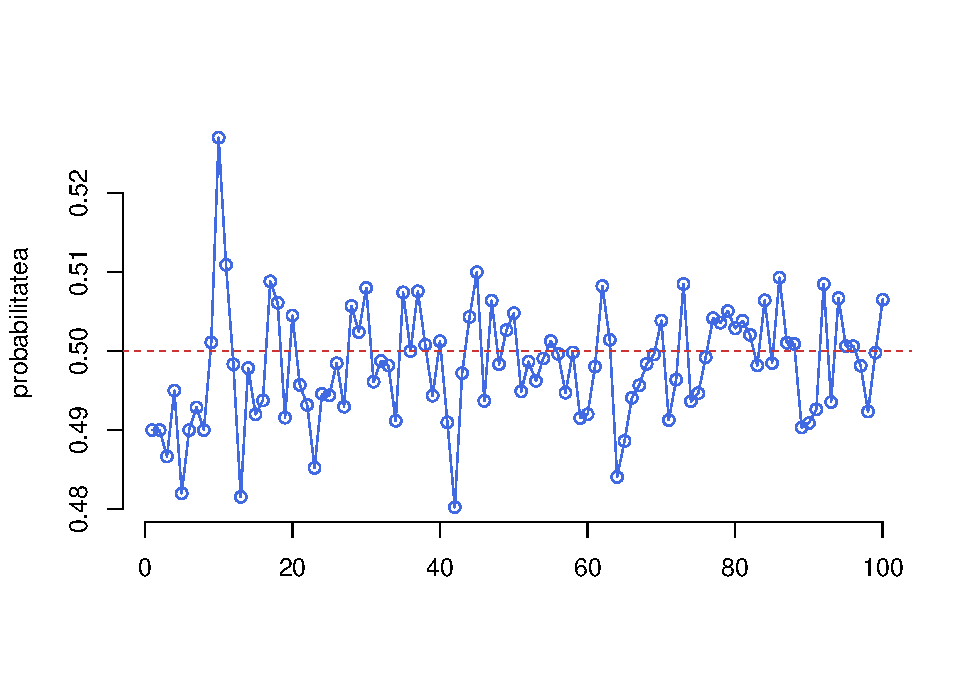
\includegraphics[width=0.8\linewidth]{Lab3_files/figure-latex/unnamed-chunk-18-1} \end{center}

\subsection{Numărul de băieți dintr-o familie cu doi
copii}\label{numarul-de-baieti-dintr-o-familie-cu-doi-copii}

\begin{rmdexercise}
O familie are doi copii. Care este probabilitatea ca ambii copii să fie
băieți știind că cel puțin unul dintre copii este băiat ? Care este
probabilitatea ca ambii copii să fie băieți știind că cel mai tânăr este
băiat ?
\end{rmdexercise}

Pentru a răspunde la cele două întrebări să observăm că cei doi copii
(copilul mai mare și cel mai mic) pot fi ambii de sex masculin sau
feminin, prin urmare avem patru combinații de sexe, pe care le
presupunem egal probabile. Putem reprezenta spațiul stărilor prin

\[
\Omega = \{BB,BF,FB,FF\}
\]

unde
\(\mathbb{P}(BB)=\mathbb{P}(BF)=\mathbb{P}(FB)=\mathbb{P}(FF)=\frac{1}{4}\).

Pentru a răspunde la prima întrebare avem:

\[
\begin{aligned}
  \mathbb{P}\left(BB\,|\,\text{cel puțin unul este băiat}\right) &= \mathbb{P}\left(BB\,|\,BF\cup FB\cup BB\right)\\
    &= \frac{\mathbb{P}\left(BB\cap (BF\cup FB\cup BB)\right)}{\mathbb{P}\left(BF\cup FB\cup BB\right)} = \frac{\mathbb{P}\left(BB\right)}{\mathbb{P}\left(BF\cup FB\cup BB\right)} = \frac{1}{3}.
\end{aligned}
\]

Iar pentru cea de-a doua întrebare:

\[
\begin{aligned}
  \mathbb{P}\left(BB\,|\,\text{cel mai tânăr este băiat}\right) &= \mathbb{P}\left(BB\,|\,FB\cup BB\right)\\
    &= \frac{\mathbb{P}\left(BB\cap (FB\cup BB)\right)}{\mathbb{P}\left(FB\cup BB\right)} = \frac{\mathbb{P}\left(BB\right)}{\mathbb{P}\left(FB\cup BB\right)} = \frac{1}{2}.
\end{aligned}
\]

Vom încerca să răspundem la aceste întrebări și cu ajutorul limbajului
R, prin simulare. Din abordarea \emph{frecvenționistă} am văzut că prin
repetarea de \(N\) ori a unui experiment în condiții identice,

\[
  \mathbb{P}(A|B)\approx \frac{N(A\cap B)}{N(B)}
\]

unde \(N(A\cap B)\) este numărul de realizări (din \(N\)) a
evenimentului \(A\cap B\) iar \(N(B)\) este numărul de realizări a
evenimentului \(B\). Să considerăm \(N = 10^5\) și fie

\begin{Shaded}
\begin{Highlighting}[]
\NormalTok{N =}\StringTok{ }\DecValTok{10}\OperatorTok{^}\DecValTok{5}

\NormalTok{copil1 =}\StringTok{ }\KeywordTok{sample}\NormalTok{(}\KeywordTok{c}\NormalTok{(}\StringTok{"baiat"}\NormalTok{, }\StringTok{"fata"}\NormalTok{), N, }\DataTypeTok{replace =} \OtherTok{TRUE}\NormalTok{)}
\NormalTok{copil2 =}\StringTok{ }\KeywordTok{sample}\NormalTok{(}\KeywordTok{c}\NormalTok{(}\StringTok{"baiat"}\NormalTok{, }\StringTok{"fata"}\NormalTok{), N, }\DataTypeTok{replace =} \OtherTok{TRUE}\NormalTok{)}
\end{Highlighting}
\end{Shaded}

Aici \texttt{copil1} este un vector de lungime \texttt{N} care
reprezintă sexul primului copil și în mod similar \texttt{copil2}
reprezintă sexul celui de-al doilea copil.

Fie \(A\) evenimentul ca ambii copii să fie băieți și \(B\) evenimentul
prin care cel mai tânăr este băiat.

\begin{Shaded}
\begin{Highlighting}[]
\NormalTok{nB =}\StringTok{ }\KeywordTok{sum}\NormalTok{(copil2 }\OperatorTok{==}\StringTok{ "baiat"}\NormalTok{)}
\NormalTok{nAB =}\StringTok{ }\KeywordTok{sum}\NormalTok{(copil1 }\OperatorTok{==}\StringTok{ "baiat"} \OperatorTok{&}\StringTok{ }\NormalTok{copil2 }\OperatorTok{==}\StringTok{ "baiat"}\NormalTok{)}

\NormalTok{p2 =}\StringTok{ }\NormalTok{nAB}\OperatorTok{/}\NormalTok{nB}
\end{Highlighting}
\end{Shaded}

Prin urmare probabilitatea (simulată) ca familia să aibă cei doi copii
băieți știind că cel tânăr este băiat este 0.4991515.

Considerând acum \(C\) evenimentul prin care familia are cel puțin un
copil băiat, avem

\begin{Shaded}
\begin{Highlighting}[]
\NormalTok{nC =}\StringTok{ }\KeywordTok{sum}\NormalTok{(copil1 }\OperatorTok{==}\StringTok{ "baiat"} \OperatorTok{|}\StringTok{ }\NormalTok{copil2 }\OperatorTok{==}\StringTok{ "baiat"}\NormalTok{)}

\NormalTok{p1 =}\StringTok{ }\NormalTok{nAB}\OperatorTok{/}\NormalTok{nC}
\end{Highlighting}
\end{Shaded}

de unde probabilitatea ca familia să aibă doar băieți știind că cel
puțin unul este băiat este 0.3339566.

\subsection{Monty Hall}\label{monty-hall}

\begin{rmdexercise}
Sunteți participant într-un joc televizat în care gazda vă prezintă trei
uși închise. Acesta vă spune că în spatele unei uși se află o mașină iar
în spatele celorlalte două se află câte o capră. Jocul decurge în felul
următor: trebuie să alegeți una dintre cele trei uși; gazda, care știe
în spatele cărei uși se află mașina, deschide una dintre celelalte două
uși, în spatele căreia se află o capră apoi vă întreabă dacă vreți să
rămâneți la alegerea inițială sau vreți să alegeți cealaltă ușă rămasă
închisă. Presupunând că vreți să câștigați o mașină, ce alegere
preferați ?
\end{rmdexercise}

Considerăm evenimentele \(C_1\), \(C_2\) și \(C_3\) ca indicând ușa în
spatele căreia se află mașina. Aceste evenimente au probabilitatea de
\(1/3\) fiecare.

Evenimentul prin care jucătorul alege ușa cu numărul 1 este notat cu
\(X_1\) și evenimentul prin care gazda deschide ușa cu numărul 3 este
notat cu \(H_3\). Avem că \(\mathbb{P}(C_i|X_1) = 1/3\) iar
\(\mathbb{P}(H_3|C_1,X_1) = 1/2\), \(\mathbb{P}(H_3|C_2,X_1) = 1\) si
\(\mathbb{P}(H_3|C_3,X_1) = 0\).

Avem că probabilitatea ca jucătorul să câștige adoptând schimbarea
ușilor este (în condițiile în care a ales inițial poarta 1 și gazda a
deschis poarta 3)

\[
\begin{aligned}
  \mathbb{P}(C_2|H_3,X_1) &= \frac{\mathbb{P}(H_3|C_2,X_1)\mathbb{P}(C_2\cap X_1)}{\mathbb{P}(H_3\cap X_1)}\\
  &=\frac{\mathbb{P}(H_3|C_2,X_1)\mathbb{P}(C_2\cap X_1)}{\mathbb{P}(H_3|C_1,X_1)\mathbb{P}(C_1\cap X_1)+\mathbb{P}(H_3|C_2,X_1)\mathbb{P}(C_2\cap X_1)+\mathbb{P}(H_3|C_3,X_1)\mathbb{P}(C_3\cap X_1)}\\
  &= \frac{\mathbb{P}(H_3|C_2,X_1)}{\mathbb{P}(H_3|C_1,X_1)+\mathbb{P}(H_3|C_2,X_1)+\mathbb{P}(H_3|C_3,X_1)} = \frac{1}{1/2+1+0} = \frac{2}{3}
\end{aligned}
\]

Intuiție (să presupunem că ne aflăm în situația în care am ales ușa cu
numărul 1):

\begin{center}
\begin{table}[ht]
\centering
  \begin{tabular}{c|c|c|c|c}
  \toprule
    Ușa 1 & Ușa 2 & Ușa 3 & Nu schimbăm & Schimbăm\\
  \midrule
    Mașină & Capră & Capră & \cmark & \xmark\\
    Capră & Mașină & Capră & \xmark & \cmark\\
    Capră & Capră & Mașină & \xmark & \cmark\\
  \bottomrule
    
  \end{tabular}
\end{table}

\end{center}

Vom încerca să simulăm jocul descris de problema noastră:

\begin{Shaded}
\begin{Highlighting}[]
\NormalTok{monty =}\StringTok{ }\ControlFlowTok{function}\NormalTok{(}\DataTypeTok{random =} \OtherTok{TRUE}\NormalTok{) \{}
\NormalTok{  doors =}\StringTok{ }\DecValTok{1}\OperatorTok{:}\DecValTok{3}
  
  \ControlFlowTok{if}\NormalTok{ (random)\{}
    \CommentTok{# alege aleator unde se afla masina}
\NormalTok{    cardoor <-}\StringTok{ }\KeywordTok{sample}\NormalTok{(doors,}\DecValTok{1}\NormalTok{)}
\NormalTok{  \}}\ControlFlowTok{else}\NormalTok{\{}
    \KeywordTok{print}\NormalTok{(}\StringTok{"Scrieti numarul usii in spatele careia se afla masina:"}\NormalTok{)}
\NormalTok{    cardoor =}\StringTok{ }\KeywordTok{scan}\NormalTok{(}\DataTypeTok{what =} \KeywordTok{integer}\NormalTok{(), }\DataTypeTok{nlines =} \DecValTok{1}\NormalTok{, }\DataTypeTok{quiet =} \OtherTok{TRUE}\NormalTok{)}
\NormalTok{  \}}
  
  \CommentTok{# Monty ii spune jucatorului sa aleaga usa }
  \KeywordTok{print}\NormalTok{(}\StringTok{"Monty Hall spune ‘Alege o usa, orice usa!’"}\NormalTok{)}
  
  \CommentTok{# alegerea jucatorului (1,2 sau 3)}
\NormalTok{  chosen =}\StringTok{ }\KeywordTok{scan}\NormalTok{(}\DataTypeTok{what =} \KeywordTok{integer}\NormalTok{(), }\DataTypeTok{nlines =} \DecValTok{1}\NormalTok{, }\DataTypeTok{quiet =} \OtherTok{TRUE}\NormalTok{)}
  
  \CommentTok{# Monty intoarce o usa cu capra (nu poate fi usa aleasa }
  \CommentTok{# de jucator si nici usa cu masina)}
  \ControlFlowTok{if}\NormalTok{ (chosen }\OperatorTok{!=}\StringTok{ }\NormalTok{cardoor)\{}
\NormalTok{     montydoor =}\StringTok{ }\NormalTok{doors[}\OperatorTok{-}\KeywordTok{c}\NormalTok{(chosen, cardoor)]}
\NormalTok{  \}}\ControlFlowTok{else}\NormalTok{\{}
\NormalTok{    montydoor =}\StringTok{ }\KeywordTok{sample}\NormalTok{(doors[}\OperatorTok{-}\NormalTok{chosen],}\DecValTok{1}\NormalTok{)}
\NormalTok{  \} }
  
  \CommentTok{# jucatorul schimba sau...}
  \KeywordTok{print}\NormalTok{(}\KeywordTok{paste}\NormalTok{(}\StringTok{"Monty deschide usa "}\NormalTok{, montydoor, }\StringTok{"!"}\NormalTok{, }\DataTypeTok{sep=}\StringTok{""}\NormalTok{))}
  \KeywordTok{print}\NormalTok{(}\StringTok{"Doresti sa schimbi usa (y/n)?"}\NormalTok{)}
  
\NormalTok{  reply =}\StringTok{ }\KeywordTok{scan}\NormalTok{(}\DataTypeTok{what =} \KeywordTok{character}\NormalTok{(), }\DataTypeTok{nlines =} \DecValTok{1}\NormalTok{, }\DataTypeTok{quiet =} \OtherTok{TRUE}\NormalTok{)}
  
  \CommentTok{# ce incepe cu "y" este da}
  \ControlFlowTok{if}\NormalTok{ (}\KeywordTok{substr}\NormalTok{(reply,}\DecValTok{1}\NormalTok{,}\DecValTok{1}\NormalTok{) }\OperatorTok{==}\StringTok{ "y"}\NormalTok{)\{}
\NormalTok{    chosen =}\StringTok{ }\NormalTok{doors[}\OperatorTok{-}\KeywordTok{c}\NormalTok{(chosen,montydoor)]}
\NormalTok{  \} }
  
  \CommentTok{# Rezultatul jocului}
  \ControlFlowTok{if}\NormalTok{ (chosen }\OperatorTok{==}\StringTok{ }\NormalTok{cardoor)\{}
    \KeywordTok{print}\NormalTok{(}\StringTok{"Bravo! Ai castigat !"}\NormalTok{)}
\NormalTok{  \}}\ControlFlowTok{else}\NormalTok{\{}
    \KeywordTok{print}\NormalTok{(}\StringTok{"Pacat! Ai pierdut!"}\NormalTok{)}
\NormalTok{  \} }
\NormalTok{\}}
\end{Highlighting}
\end{Shaded}

\subsection{Jocul de loto}\label{jocul-de-loto}

\begin{rmdexercise}
Construiți în R o funcție care să simuleze jocul de loto \(6/49\). Acest
joc consistă din extragerea aleatoare a \(6\) numere dintr-o urnă cu
\(49\) de numere posibile, fără întoarcere. Fiecare extragere se face de
manieră uniformă din numerele rămase în urnă (la a i-a extragere fiecare
bilă din urnă are aceeași șansă să fie extrasă). De exemplu putem avea
următorul rezultat: \(10, 27, 3, 45, 12, 24\).

\textbf{Notă}: Funcția \texttt{sample()} poate face această operație,
ceea ce se cere este de a crea voi o funcție care să implementeze jocul
fără a folosi funcția \emph{sample}. Binențeles că puteți folosi funcții
precum: \texttt{runif} , \texttt{floor}, \texttt{choose}, etc.
\end{rmdexercise}

Începem prin a construi o funcție care ne permite generarea unei
variabile aleatoare uniform repartizate pe mulțimea \(\{1,2,\dots,n\}\)
(această funcție este cea care simulează procesul de extragere de la
fiecare pas):

\begin{Shaded}
\begin{Highlighting}[]
\NormalTok{myintunif =}\StringTok{ }\ControlFlowTok{function}\NormalTok{(n)\{}
  \CommentTok{# dunctia care genereaza un numar uniform intre 1 si n}
\NormalTok{  r =}\StringTok{ }\NormalTok{n}\OperatorTok{*}\KeywordTok{runif}\NormalTok{(}\DecValTok{1}\NormalTok{)}
\NormalTok{  u =}\StringTok{ }\KeywordTok{floor}\NormalTok{(r)}\OperatorTok{+}\DecValTok{1}
  \KeywordTok{return}\NormalTok{(u)}
\NormalTok{\}}
\end{Highlighting}
\end{Shaded}

Funcția care realizează extragerea fără întoarcere a \(k\) numere
aleatoare din \(n\), este:

\begin{Shaded}
\begin{Highlighting}[]
\NormalTok{myrandsample=}\ControlFlowTok{function}\NormalTok{(n,k)\{}
  \CommentTok{# }
\NormalTok{  x =}\StringTok{ }\DecValTok{1}\OperatorTok{:}\NormalTok{n}
\NormalTok{  q =}\StringTok{ }\KeywordTok{rep}\NormalTok{(}\DecValTok{0}\NormalTok{,k)}
  
  \ControlFlowTok{for}\NormalTok{(i }\ControlFlowTok{in} \DecValTok{1}\OperatorTok{:}\NormalTok{k)\{}
\NormalTok{    l =}\StringTok{ }\KeywordTok{length}\NormalTok{(x)}
\NormalTok{    u =}\StringTok{ }\KeywordTok{myintunif}\NormalTok{(l)}
\NormalTok{    q[i] =}\StringTok{ }\NormalTok{x[u]}
\NormalTok{    x =}\StringTok{ }\NormalTok{x[x}\OperatorTok{!=}\NormalTok{q[i]]}
\NormalTok{  \}}
  \KeywordTok{return}\NormalTok{(q)}
\NormalTok{\}}
\end{Highlighting}
\end{Shaded}

Pentru a vedea ce face această funcție putem scrie:

\begin{Shaded}
\begin{Highlighting}[]
\NormalTok{n =}\StringTok{ }\DecValTok{49}
\NormalTok{k =}\StringTok{ }\DecValTok{6}

\KeywordTok{myrandsample}\NormalTok{(n,k)}
\NormalTok{[}\DecValTok{1}\NormalTok{] }\DecValTok{28} \DecValTok{19} \DecValTok{43}  \DecValTok{1} \DecValTok{41} \DecValTok{39}
\end{Highlighting}
\end{Shaded}

\section{Aplicația 1: Verificarea egalității a două
polinoame}\label{aplicatia-1-verificarea-egalitatii-a-doua-polinoame}

În această secțiune ne propunem să abordăm următoarea problemă:

\begin{rmdexercise}
Având date două polinoame \(F(x)\) și \(G(x)\), cu
\(F(x)=\prod_{i=1}^d(x-a_i)\) și \(G(x)\) dat sub forma canonică
(\(\sum_{i=0}^d c_ix^i\)), vrem să verificăm dacă are loc identitatea

\[
  F(x) \overset{?}{\equiv} G(x).
\]
\end{rmdexercise}

Știm că două polinoame sunt egale atunci când coeficienții lor în
descompunerea canonică sunt egali. Observăm că dacă am transforma
polinonum \(F(x)\) la forma sa canonică prin înmulțirea consecutivă a
monomului \(i\) cu produsul primelor \(i-1\) monoame atunci am avea
nevoie de \(\Theta(d^2)\) operații. În cele ce urmează presupunem că
fiecare operație de înmulțire se poate face în timp constant, ceea ce nu
corespunde în totalitate cu realitatea în special în cazurile în care
vrem să înmulțim coeficienți mari.

Ne propunem să construim un algoritm randomizat care să verifice această
egalitate într-un număr mai mic de operații (\(O(d)\) operații). Să
presupunem că \(d\) este gradul maxim al lui \(x\) (exponentul cel mai
mare) în \(F(x)\) și \(G(x)\). Algoritmul poate fi descris astfel:
alegem uniform un număr \(r\) din mulțimea \(\{1,2,\ldots,100d\}\) (prin
uniform înțelegem că cele \(100d\) numere au aceeași șansă să fie alese)
și calculăm valorile lui \(F(r)\) și \(G(r)\). Dacă \(F(r)\neq G(r)\)
atunci algoritmul întoarce că cele două polinoame nu sunt egale iar dacă
\(F(r)=G(r)\) atunci algoritmul întoarce că cele două polinoame sunt
egale. Algoritmul poate greși doar dacă cele două polinoame nu sunt
egale dar \(F(r)=G(r)\). Vrem să evaluăm această probabilitate.

Experimentul nostru poate fi modelat cu ajutorul tripletului
\((\Omega, \mathcal{F}, \mathbb{P})\) unde
\(\Omega = \{1,2,\ldots,100d\}\), \(\mathcal{F}=\mathcal{P}(\Omega)\)
iar \(\mathbb{P}\) este echirepartiția pe \(\Omega\). Fie \(E\)
evenimentul că algoritmul greșește, acest eveniment se realizează doar
dacă numărul aleator \(r\) este o rădăcină a polinomului \(F(x)-G(x)\),
de grad cel mult \(d\). Cum din \emph{Teorema Fundamentală a Algebrei}
acest polinom nu poate avea mai mult de \(d\) rădăcini rezultă că

\[
  \mathbb{P}(\text{algoritmul greseste}) = \mathbb{P}(E) \leq \frac{d}{100d} = \frac{1}{100}.
\]

Putem să îmbunătățim această probabilitate? O variantă ar fi să mărim
spațiul stărilor la \(\Omega = \{1,2,\ldots,1000d\}\) și atunci șansa ca
algoritmul să greșească ar fi de \(\frac{1}{1000}\). O altă variantă ar
fi să repetăm procedeul de mai multe ori, iar în această situație
algoritmul ar fi eronat doar dacă ar întoarce că cele două polinoame
sunt egale când în realitate ele nu sunt. Atunci când repetăm procesul,
alegerea numărului aleator \(r\) se poate face în două moduri diferite:
cu întoarcere (nu ținem cont de numerele ieșite) sau fără întoarcere
(ținem cont de numerele ieșite).

Dacă luăm \(E_i\) evenimentul prin care la a i-a rulare a algoritmului
am extras o rădăcină \(r_i\) astfel încât \(F(r_i)=G(r_i)\), atunci
probabilitatea ca algoritmul să întoarcă un răspuns greșit după \(k\)
repetări, este

\[
  \mathbb{P}(E_1\cap E_2\cap \cdots\cap E_k).
\]

În cazul în care alegerea se face cu întoarcere (evenimentele sunt
independente) obținem

\[
  \mathbb{P}(E_1\cap E_2\cap \cdots\cap E_k) = \prod_{i=1}^{k}\mathbb{P}(E_i)\leq\prod_{i=1}^{k}\frac{d}{100d} = \left(\frac{1}{100}\right)^k,
\]

iar dacă extragerea s-a făcut fără întoarcere (evenimentele nu mai sunt
independente), atunci folosind regula de multiplicare avem

\begin{align*}
  \mathbb{P}(E_1\cap E_2\cap \cdots\cap E_k) &= \mathbb{P}(E_1)\mathbb{P}(E_2|E_1)\cdots\mathbb{P}(E_k|E_1\cap\cdots\cap E_{k-1})\\
                    &\leq \prod_{i=1}^{k}\frac{d - (i-1)}{100d - (i-1)} \leq \left(\frac{1}{100}\right)^k.
\end{align*}

\begin{Shaded}
\begin{Highlighting}[]
\NormalTok{Fx =}\StringTok{ }\ControlFlowTok{function}\NormalTok{(x)\{}
  \KeywordTok{return}\NormalTok{((x}\OperatorTok{+}\DecValTok{1}\NormalTok{)}\OperatorTok{*}\NormalTok{(x}\OperatorTok{-}\DecValTok{2}\NormalTok{)}\OperatorTok{*}\NormalTok{(x}\OperatorTok{+}\DecValTok{3}\NormalTok{)}\OperatorTok{*}\NormalTok{(x}\OperatorTok{-}\DecValTok{4}\NormalTok{)}\OperatorTok{*}\NormalTok{(x}\OperatorTok{+}\DecValTok{5}\NormalTok{)}\OperatorTok{*}\NormalTok{(x}\OperatorTok{-}\DecValTok{6}\NormalTok{))}
\NormalTok{\}}

\NormalTok{Gx =}\StringTok{ }\ControlFlowTok{function}\NormalTok{(x)\{}
  \KeywordTok{return}\NormalTok{(x}\OperatorTok{^}\DecValTok{6} \OperatorTok{-}\StringTok{ }\DecValTok{7}\OperatorTok{*}\NormalTok{x}\OperatorTok{^}\DecValTok{3} \OperatorTok{+}\StringTok{ }\DecValTok{25}\NormalTok{)}
\NormalTok{\}}

\NormalTok{Gx2 =}\StringTok{ }\ControlFlowTok{function}\NormalTok{(x)\{}
  \KeywordTok{return}\NormalTok{(x}\OperatorTok{^}\DecValTok{6} \OperatorTok{-}\StringTok{ }\DecValTok{3}\OperatorTok{*}\NormalTok{x}\OperatorTok{^}\DecValTok{5} \OperatorTok{-}\StringTok{ }\DecValTok{41}\OperatorTok{*}\NormalTok{x}\OperatorTok{^}\DecValTok{4} \OperatorTok{+}\StringTok{ }\DecValTok{87}\OperatorTok{*}\NormalTok{x}\OperatorTok{^}\DecValTok{3} \OperatorTok{+}\StringTok{ }\DecValTok{400}\OperatorTok{*}\NormalTok{x}\OperatorTok{^}\DecValTok{2} \OperatorTok{-}\StringTok{ }\DecValTok{444}\OperatorTok{*}\NormalTok{x }\OperatorTok{-}\StringTok{ }\DecValTok{720}\NormalTok{)}
\NormalTok{\}}

\NormalTok{comparePols =}\StringTok{ }\ControlFlowTok{function}\NormalTok{(Fx, Gx)\{}
\NormalTok{  k =}\StringTok{ }\DecValTok{3} \CommentTok{# repetam algoritmul de 3 ori}
\NormalTok{  d =}\StringTok{ }\DecValTok{6} \CommentTok{# gradul polinomului }
  
  \ControlFlowTok{for}\NormalTok{ (i }\ControlFlowTok{in} \DecValTok{1}\OperatorTok{:}\NormalTok{k)\{}
\NormalTok{    r =}\StringTok{ }\KeywordTok{floor}\NormalTok{(}\DecValTok{100}\OperatorTok{*}\NormalTok{d}\OperatorTok{*}\KeywordTok{runif}\NormalTok{(}\DecValTok{1}\NormalTok{)) }\OperatorTok{+}\StringTok{ }\DecValTok{1}
    
\NormalTok{    f1 =}\StringTok{ }\KeywordTok{Fx}\NormalTok{(r)}
\NormalTok{    g1 =}\StringTok{ }\KeywordTok{Gx}\NormalTok{(r)}
    
    \ControlFlowTok{if}\NormalTok{ (f1}\OperatorTok{!=}\NormalTok{g1)\{}
      \KeywordTok{return}\NormalTok{(}\KeywordTok{cat}\NormalTok{(}\StringTok{"Cele doua polinoame sunt diferite ! }\CharTok{\textbackslash{}n}\StringTok{Pentru r ="}\NormalTok{, }
\NormalTok{                         r, }\StringTok{"avem ca F(r)!=G(r) ("}\NormalTok{, f1, }\StringTok{"!="}\NormalTok{, g1, }\StringTok{")"}\NormalTok{))}
\NormalTok{    \}}
    
\NormalTok{  \}}
  
  \KeywordTok{return}\NormalTok{(}\KeywordTok{cat}\NormalTok{(}\StringTok{"Polinoamele sunt egale. Eroarea este de"}\NormalTok{, }\DecValTok{100}\OperatorTok{^}\NormalTok{(}\OperatorTok{-}\NormalTok{k)))}
\NormalTok{\}}

\KeywordTok{comparePols}\NormalTok{(Fx, Gx)}
\NormalTok{Cele doua polinoame sunt diferite }\OperatorTok{!}\StringTok{ }
\NormalTok{Pentru r =}\StringTok{ }\DecValTok{246}\NormalTok{ avem ca }\KeywordTok{F}\NormalTok{(r)}\OperatorTok{!=}\KeywordTok{G}\NormalTok{(r) ( }\FloatTok{2.187693e+14} \OperatorTok{!=}\StringTok{ }\FloatTok{2.216208e+14}\NormalTok{ )}

\KeywordTok{comparePols}\NormalTok{(Fx, Gx2)}
\NormalTok{Polinoamele sunt egale. Eroarea este de }\FloatTok{1e-06}
\end{Highlighting}
\end{Shaded}

\section{Aplicația 2: Verificarea produsului a două
matrice}\label{aplicatia-2-verificarea-produsului-a-doua-matrice}

În cele ce urmează vom prezenta o altă aplicație în care algoritmul
randomizat este mult mai eficient decât orice algoritm determinist
cunoscut până în acest moment.

\begin{rmdexercise}
Să presupunem că avem trei matrice pătratice \(\bf{A}\), \(\bf{B}\) și
\(\bf{C}\) de dimensiune \(n \times n\). Pentru simplitate considerăm că
avem de-a face cu matrice cu elemente de \(0\) și \(1\) iar operațiile
se fac \(\mod2\). Vrem să construim un algoritm randomizat care să
verifice egalitatea: \[
  \bf{A}\cdot\bf{B}=\bf{C} \qquad (\text{mod 2}).
\]
\end{rmdexercise}

O modalitate ar fi să calculăm elementele matricii
\(\bf{C}'=\bf{A}\cdot\bf{B}\), folosind relația
\(C'_{i,j} = \sum_{k=1}^{n}A_{i,k}B_{k,j}\), și să le comparăm cu
elementele matricii \(\bf{C}\). Metoda \emph{naivă} de multiplicare a
celor două matrice necesită cel mult \(O(n^3)\) operații. Știm că există
algoritmi (netriviali) care permit multiplicarea matricelor într-un
număr mai mic de operații, ca de exemplu:

\begin{rmdinsight}
(Strassen 1969) Este posibil să înmulțim două matrice în aproape
\(n^{\log_27}\approx n^{2.81}\) operații.
\end{rmdinsight}

iar o versiune îmbunătățită a algoritmului lui Strassen (și cea care
deținea recordul până în 2014\footnote{Actualul record este
  \(O(n^{2.3728})\) dat de
  \href{http://theory.stanford.edu/~virgi/matrixmult-f.pdf}{Vassilevska
  Williams}})

\begin{rmdinsight}
(Coppersmith-Winograd 1987) Este posibil să înmulțim două matrice în
aproape \(n^{2.376}\) operații.
\end{rmdinsight}

Noi nu vom vorbi despre algoritmi de multiplicare a două matrice, ci de
algoritmi de verificare a acestei operații. Pentru aceasta vom considera
un algoritm randomizat care verifică înmulțirea în aproximativ \(n^2\)
operații (\(O(n^2)\)) cu precizarea că acest algoritm poate conduce la
un răspuns eronat.

\begin{rmdinsight}
(Freivalds 1979) Există un algoritm probabilist care poate verifica dacă
\(\bf{A}\cdot\bf{B}=\bf{C} \quad (\text{mod 2})\) în \(O(n^2)\) operații
și având o eroare de \(2^{-200}\).
\end{rmdinsight}

Algoritmul lui de bază a lui Freivalds este următorul:

\begin{enumerate}
\def\labelenumi{\arabic{enumi}.}
\item
  Alegem uniform un vector \(\bf{r}=(r_1,r_2,\ldots,r_n)\in\{0,1\}^n\)
  (unde prin ales uniform înțelegem că fiecare \(r_i\) este ales de
  manieră independentă cu probabilitatea de \(0.5\) să ia valoarea \(0\)
  sau \(1\)\footnote{Putem să ne imaginăm că aruncăm cu un ban
    echilibrat de \(n\) ori și convertim capul în \(1\) și pajura în
    \(0\).})
\item
  Calculăm \(y = \bf{A}\bf{B}\bf{r}\) și \(z = \bf{C}\bf{r}\). Dacă
  \(y = z\) atunci algoritmul întoarce \emph{multiplicarea este corectă}
  altfel \emph{multiplicarea matricelor este eronată}.
\end{enumerate}

Observăm că acest algoritm necesită trei operații de multiplicare între
o matrice și un vector, prin urmare acesta necesită \(O(n^2)\) pași. De
asemenea, remarcăm că algoritmul întoarce un răspuns eronat atunci când
\(\bf{A}\cdot\bf{B}\neq\bf{C}\) dar
\(\bf{A}\bf{B}\bf{r} = \bf{C}\bf{r}\). Probabilitatea ca algoritmul să
întoarcă un raspuns eronat verifică

\[
  \mathbb{P}(\text{algoritmul intoarce raspuns gresit}) = \mathbb{P}(\bf{A}\bf{B}\bf{r} = \bf{C}\bf{r}) \leq \frac{1}{2}.
\]

Pentru a verifica acest rezultat, fie
\(\bf{D} = \bf{A}\cdot\bf{B}-\bf{C} \neq 0\). Evenimentul
\(\{\bf{A}\bf{B}\bf{r} = \bf{C}\bf{r}\}\) implică \(\bf{D}\bf{r}=0\) și
cum \(\bf{D}\neq 0\) putem presupune că elementul \(d_{1,1}\neq 0\).
Deoarece \(\bf{D}\bf{r}=0\) rezultă că \(\sum_{j=1}^{n}d_{1,j}r_j=0\)
sau, echivalent

\[
  r_1 = -\frac{\sum_{j=2}^{n}d_{1,j}r_j}{d_{1,1}}.
\] Avem

\begin{align*}
  \mathbb{P}(\bf{A}\bf{B}\bf{r} = \bf{C}\bf{r}) &= \sum_{(x_2,\cdots, x_n)\in\{0,1\}^n}\mathbb{P}\left(\{\bf{A}\bf{B}\bf{r} = \bf{C}\bf{r}\}\cap \{(r_2,\cdots, r_n) = (x_2,\cdots, x_n)\}\right)\\
      &\leq \sum_{(x_2,\cdots, x_n)\in\{0,1\}^n}\mathbb{P}\left(\left\{r_1 = -\frac{\sum_{j=2}^{n}d_{1,j}r_j}{d_{1,1}}\right\}\cap \{(r_2,\cdots, r_n) = (x_2,\cdots, x_n)\}\right)\\
      &\leq \sum_{(x_2,\cdots, x_n)\in\{0,1\}^n}\mathbb{P}\left(\left\{r_1 = -\frac{\sum_{j=2}^{n}d_{1,j}r_j}{d_{1,1}}\right\}\right)\mathbb{P}\left(\{(r_2,\cdots, r_n) = (x_2,\cdots, x_n)\}\right)\\
      &\leq \sum_{(x_2,\cdots, x_n)\in\{0,1\}^n}\frac{1}{2}\mathbb{P}\left(\{(r_2,\cdots, r_n) = (x_2,\cdots, x_n)\}\right)\\
      &= \frac{1}{2}.
\end{align*}

În relațiile de mai sus am folosit faptul că \(r_1\) și
\((r_2,\cdots, r_n)\) sunt independente.

Pentru a îmbunătății eroarea algoritmului putem să repetăm procedeul de
\(k\) ori\footnote{Algoritmul lui Freivalds presupune \(k = 200\).} și
în acest caz probabilitatea de eroare devine \(2^{-k}\) iar numărul de
operații \(O(kn^2)\).

\begin{Shaded}
\begin{Highlighting}[]

\NormalTok{FreivaldsAlg =}\StringTok{ }\ControlFlowTok{function}\NormalTok{(A, B, C)\{}
  \CommentTok{# Algoritmul Freivalds}
\NormalTok{  n =}\StringTok{ }\KeywordTok{dim}\NormalTok{(A)[}\DecValTok{1}\NormalTok{] }\CommentTok{# dimensiunea matricelor}
  
\NormalTok{  k =}\StringTok{ }\KeywordTok{ceiling}\NormalTok{(}\KeywordTok{log}\NormalTok{(n)) }\CommentTok{# numarul de repetari ale algoritmului}
  
  \ControlFlowTok{for}\NormalTok{ (i }\ControlFlowTok{in} \DecValTok{1}\OperatorTok{:}\NormalTok{k)\{}
\NormalTok{    r =}\StringTok{ }\KeywordTok{rbinom}\NormalTok{(n, }\DecValTok{1}\NormalTok{, }\DataTypeTok{prob =} \FloatTok{0.5}\NormalTok{)}
    
\NormalTok{    y =}\StringTok{ }\NormalTok{B}\OperatorTok\NormalTok{r}
\NormalTok{    y =}\StringTok{ }\NormalTok{A}\OperatorTok\NormalTok{y}
\NormalTok{    y =}\StringTok{ }\NormalTok{y}\OperatorTok\DecValTok{2}
    
\NormalTok{    z =}\StringTok{ }\NormalTok{C}\OperatorTok\NormalTok{r}
\NormalTok{    z =}\StringTok{ }\NormalTok{z}\OperatorTok\DecValTok{2}
    
    \ControlFlowTok{if}\NormalTok{ (}\KeywordTok{any}\NormalTok{(y }\OperatorTok{!=}\StringTok{ }\NormalTok{z))\{}
      \KeywordTok{return}\NormalTok{(}\KeywordTok{print}\NormalTok{(}\StringTok{"Multiplicarea matricelor este incorecta!"}\NormalTok{))}
\NormalTok{    \}}
    
\NormalTok{  \}}
  
  \KeywordTok{return}\NormalTok{(}\KeywordTok{cat}\NormalTok{(}\StringTok{"Multiplicarea matricelor este corecta!}
\StringTok{             }\CharTok{\textbackslash{}n}\StringTok{Probabilitatea de eroare a algoritmului este"}\NormalTok{, }\DecValTok{2}\OperatorTok{^}\NormalTok{\{}\OperatorTok{-}\NormalTok{k\}))}
\NormalTok{\}}

\CommentTok{# Exemplul 1}
\KeywordTok{set.seed}\NormalTok{(}\DecValTok{1234}\NormalTok{)}
\NormalTok{A =}\StringTok{ }\KeywordTok{matrix}\NormalTok{(}\KeywordTok{rbinom}\NormalTok{(}\DecValTok{225}\NormalTok{, }\DecValTok{1}\NormalTok{, }\FloatTok{0.5}\NormalTok{), }\DataTypeTok{nrow =} \DecValTok{15}\NormalTok{)}
\NormalTok{B =}\StringTok{ }\KeywordTok{matrix}\NormalTok{(}\KeywordTok{rbinom}\NormalTok{(}\DecValTok{225}\NormalTok{, }\DecValTok{1}\NormalTok{, }\FloatTok{0.5}\NormalTok{), }\DataTypeTok{nrow =} \DecValTok{15}\NormalTok{)}

\NormalTok{C =}\StringTok{ }\NormalTok{A}\OperatorTok\NormalTok{B}
\NormalTok{C =}\StringTok{ }\NormalTok{C}\OperatorTok\DecValTok{2}

\KeywordTok{FreivaldsAlg}\NormalTok{(A, B, C)}
\NormalTok{Multiplicarea matricelor este corecta}\OperatorTok{!}
\StringTok{             }
\NormalTok{Probabilitatea de eroare a algoritmului este }\FloatTok{0.125}

\CommentTok{# Exemplul 2}
\KeywordTok{set.seed}\NormalTok{(}\DecValTok{5678}\NormalTok{)}
\NormalTok{A1 =}\StringTok{ }\KeywordTok{matrix}\NormalTok{(}\KeywordTok{rbinom}\NormalTok{(}\DecValTok{625}\NormalTok{, }\DecValTok{1}\NormalTok{, }\FloatTok{0.5}\NormalTok{), }\DataTypeTok{nrow =} \DecValTok{25}\NormalTok{)}
\NormalTok{B1 =}\StringTok{ }\KeywordTok{matrix}\NormalTok{(}\KeywordTok{rbinom}\NormalTok{(}\DecValTok{625}\NormalTok{, }\DecValTok{1}\NormalTok{, }\FloatTok{0.5}\NormalTok{), }\DataTypeTok{nrow =} \DecValTok{25}\NormalTok{)}

\NormalTok{C1 =}\StringTok{ }\NormalTok{A1}\OperatorTok\KeywordTok{t}\NormalTok{(B1)}
\NormalTok{C1 =}\StringTok{ }\NormalTok{C1}\OperatorTok\DecValTok{2}

\NormalTok{C2 =}\StringTok{ }\NormalTok{A1}\OperatorTok\NormalTok{B1}
\NormalTok{C2 =}\StringTok{ }\NormalTok{C2}\OperatorTok\DecValTok{2}

\KeywordTok{FreivaldsAlg}\NormalTok{(A1, B1, C1)}
\NormalTok{[}\DecValTok{1}\NormalTok{] }\StringTok{"Multiplicarea matricelor este incorecta!"}
\KeywordTok{FreivaldsAlg}\NormalTok{(A1, B1, C2)}
\NormalTok{Multiplicarea matricelor este corecta}\OperatorTok{!}
\StringTok{             }
\NormalTok{Probabilitatea de eroare a algoritmului este }\FloatTok{0.0625}

\CommentTok{# Exemplul 3}
\KeywordTok{set.seed}\NormalTok{(}\DecValTok{5678910}\NormalTok{)}
\NormalTok{A3 =}\StringTok{ }\KeywordTok{matrix}\NormalTok{(}\KeywordTok{rbinom}\NormalTok{(}\DecValTok{1000000}\NormalTok{, }\DecValTok{1}\NormalTok{, }\FloatTok{0.5}\NormalTok{), }\DataTypeTok{nrow =} \DecValTok{1000}\NormalTok{)}
\NormalTok{B3 =}\StringTok{ }\KeywordTok{matrix}\NormalTok{(}\KeywordTok{rbinom}\NormalTok{(}\DecValTok{1000000}\NormalTok{, }\DecValTok{1}\NormalTok{, }\FloatTok{0.5}\NormalTok{), }\DataTypeTok{nrow =} \DecValTok{1000}\NormalTok{)}

\NormalTok{C3 =}\StringTok{ }\NormalTok{A3}\OperatorTok\NormalTok{B3}
\NormalTok{C3 =}\StringTok{ }\NormalTok{C3}\OperatorTok\DecValTok{2}

\KeywordTok{FreivaldsAlg}\NormalTok{(A3, B3, C3)}
\NormalTok{Multiplicarea matricelor este corecta}\OperatorTok{!}
\StringTok{             }
\NormalTok{Probabilitatea de eroare a algoritmului este }\FloatTok{0.0078125}
\end{Highlighting}
\end{Shaded}


\end{document}
